\documentclass[tikz,border=0pt]{standalone}
% Shared publication style. Compile figure sources from this directory.
\usepackage[T1]{fontenc}
\usepackage{lmodern}
\usepackage{amsmath,amssymb}
\usepackage{tikz}
\usepackage{pgfplots}
\usetikzlibrary{arrows.meta,calc,positioning,backgrounds,patterns,shapes.geometric}
\usepgfplotslibrary{groupplots,fillbetween}
\pgfplotsset{compat=1.18}
\definecolor{fgblue}{HTML}{0072B2}
\definecolor{fgorange}{HTML}{D55E00}
\definecolor{fgslate}{HTML}{8B949E}
\definecolor{fgdark}{HTML}{25313C}
\definecolor{fgpale}{HTML}{F2F6F8}
\definecolor{fggrid}{HTML}{E3E8EC}
\definecolor{fgwater}{HTML}{D6EAF4}
\definecolor{fgland}{HTML}{E8E3D3}
\renewcommand{\familydefault}{\sfdefault}
\tikzset{every picture/.style={font=\fontsize{9}{11}\selectfont,text=fgdark},
  panel label/.style={font=\bfseries\fontsize{10}{12}\selectfont,anchor=north west},
  panel title/.style={font=\bfseries\fontsize{9}{11}\selectfont,anchor=north west},
  light arrow/.style={-{Stealth[length=1.6mm]},draw=fgslate,line width=.65pt}}
\pgfplotsset{fg axis/.style={
  axis line style={fgslate,line width=.4pt},axis x line*=bottom,axis y line*=left,
  tick align=outside,tick style={fgslate,line width=.4pt},
  tick label style={font=\fontsize{8}{10}\selectfont,text=fgdark},
  label style={font=\fontsize{9}{11}\selectfont,text=fgdark},
  title style={font=\bfseries\fontsize{9}{11}\selectfont,text=fgdark},
  grid style={fggrid,line width=.35pt},minor tick num=0,
  legend style={draw=none,fill=none,font=\fontsize{8}{10}\selectfont},
  scaled ticks=false,clip=false,
  every axis plot/.append style={line width=.85pt,mark size=2.2pt}
}}

% Conceptual artwork only. The two birds are the same reusable vector drawing;
% they are not Waterbirds samples or reconstructions of experimental images.
\newcommand{\waterbird}[2]{%
  \begin{scope}[shift={(#1,#2)}]
    % Complete foreground, reused without any change between environments.
    \path[fill=fgdark] (-10,2) .. controls (-7,1) and (-6,1) .. (-4,2)
      .. controls (0,4) and (3,3) .. (5,4)
      .. controls (7,6) and (5,10) .. (7,11)
      .. controls (10,13) and (13,11) .. (12,8)
      .. controls (10,7) and (9,5) .. (9,2)
      .. controls (8,-3) and (-6,-4) .. (-10,2) -- cycle;
    \path[fill=white] (-9,1.5) .. controls (-5,1) and (-2,1) .. (0,2)
      .. controls (4,2) and (6,1) .. (7,4)
      .. controls (7,6) and (8,8) .. (9.5,8)
      .. controls (9,5) and (11,1) .. (7,-1)
      .. controls (1,-4) and (-7,-2) .. (-9,1.5) -- cycle;
    \path[fill=fgslate!70!fgdark] (-6,1) .. controls (-2,4) and (4,4) .. (5,1)
      .. controls (1,-1) and (-3,-1) .. (-6,1) -- cycle;
    \draw[white!65!fgslate,line width=.4pt] (-4,.7) .. controls (-1,2.1) and (2,2.4) .. (3.8,1.6);
    \path[fill=fgorange!85] (11.6,9.3) -- (16,8.5) -- (11.5,7.9) -- cycle;
    \fill[white] (10.1,10) circle[radius=.53];
    \fill[fgdark] (10.25,10) circle[radius=.27];
  \end{scope}}
\begin{document}
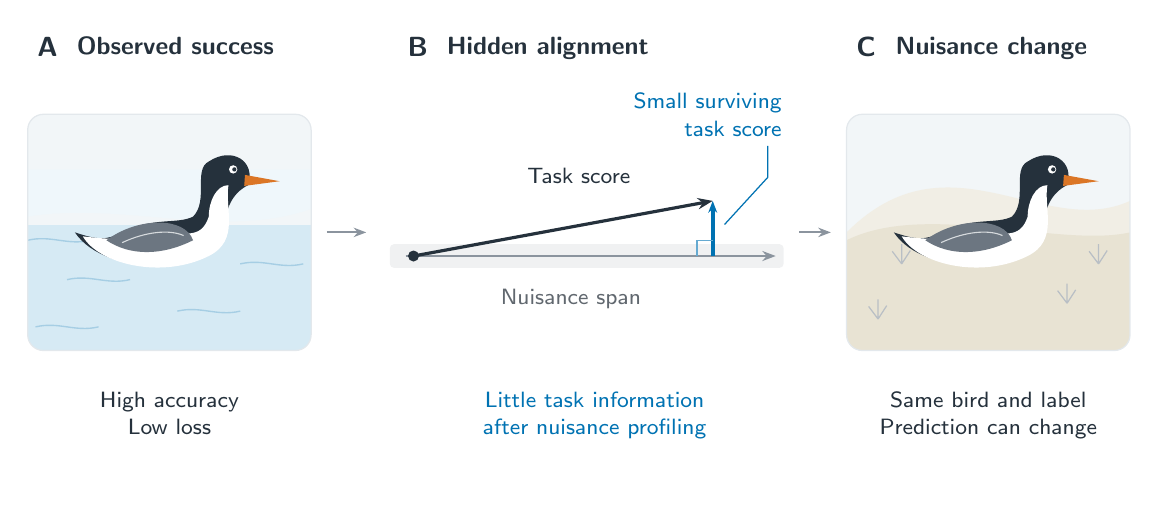
\begin{tikzpicture}[x=1mm,y=1mm]
\path[use as bounding box] (0,0) rectangle (140,57);
\node[panel label] at (0,57) {A};
\node[panel title] at (5,57) {Observed success};
\node[panel label] at (47,57) {B};
\node[panel title] at (52,57) {Hidden alignment};
\node[panel label] at (104,57) {C};
\node[panel title] at (109,57) {Nuisance change};

% Two restrained landscape illustrations, with the same foreground macro.
\begin{scope}
  \clip[rounded corners=2mm] (0,16) rectangle (36,46);
  \fill[fgpale] (0,16) rectangle (36,46);
  \fill[fgwater] (0,16) rectangle (36,32);
  \path[fill=fgwater!40] (0,33) .. controls (12,35) and (25,30) .. (36,34) -- (36,39) -- (0,39) -- cycle;
  \foreach \xx/\yy in {1/19,19/21,5/25,27/27,0/30}{
    \draw[fgblue!35,line width=.5pt] (\xx,\yy) .. controls +(3,.7) and +(-3,-.7) .. +(8,0);}
  \waterbird{16}{29}
\end{scope}
\draw[fggrid,rounded corners=2mm,line width=.45pt] (0,16) rectangle (36,46);

% A vector decomposition, without numerical axes or a data plot.
\path[fill=fgslate!13,rounded corners=.5mm] (46,26.5) rectangle (96,29.5);
\draw[fgslate,line width=.7pt,-{Stealth[length=1.7mm]}] (48,28) -- (95,28);
\draw[fgdark,line width=1.15pt,-{Stealth[length=1.9mm]}] (49,28) -- (87,35);
\draw[fgblue,line width=1.6pt,-{Stealth[length=1.5mm]}] (87,28) -- (87,35);
\draw[fgblue!60,line width=.45pt] (85,28) -- (85,30) -- (87,30);
\fill[fgdark] (49,28) circle[radius=.7];
\node[anchor=south,font=\fontsize{8}{10}\selectfont] at (70,36) {Task score};
\node[anchor=north,font=\fontsize{8}{10}\selectfont,text=fgslate!70!black] at (69,25) {Nuisance span};
\draw[fgblue,line width=.45pt] (88.5,32) -- (94,38) -- (94,42);
\node[anchor=south east,font=\fontsize{8}{10}\selectfont,text=fgblue,align=right] at (97,42) {Small surviving\\task score};

\begin{scope}
  \clip[rounded corners=2mm] (104,16) rectangle (140,46);
  \fill[fgpale] (104,16) rectangle (140,46);
  \path[fill=fgland!60] (104,31) .. controls (117,44) and (129,30) .. (140,35) -- (140,16) -- (104,16) -- cycle;
  \path[fill=fgland] (104,16) -- (104,30) .. controls (114,35) and (131,29) .. (140,31) -- (140,16) -- cycle;
  \foreach \xx/\yy in {108/20,132/22,136/27,111/27}{
    \draw[fgslate!60,line width=.45pt] (\xx,\yy) -- +(0,2.5) (\xx,\yy) -- +(-1.2,1.6) (\xx,\yy) -- +(1.1,1.7);}
  \waterbird{120}{29}
\end{scope}
\draw[fggrid,rounded corners=2mm,line width=.45pt] (104,16) rectangle (140,46);

\draw[light arrow] (38,31) -- (43,31);
\draw[light arrow] (98,31) -- (102,31);
\node[anchor=north,align=center,font=\fontsize{8}{10}\selectfont] at (18,12) {High accuracy\\Low loss};
\node[anchor=north,align=center,font=\fontsize{8}{10}\selectfont,text=fgblue] at (72,12) {Little task information\\after nuisance profiling};
\node[anchor=north,align=center,font=\fontsize{8}{10}\selectfont] at (122,12) {Same bird and label\\Prediction can change};
\end{tikzpicture}
\end{document}
